\documentclass[12pt,letterpaper]{article}
\usepackage{graphicx,textcomp}
\usepackage{natbib}
\usepackage{setspace}
\usepackage{fullpage}
\usepackage{color}
\usepackage[reqno]{amsmath}
\usepackage{amsthm}
\usepackage{fancyvrb}
\usepackage{amssymb,enumerate}
\usepackage[all]{xy}
\usepackage{endnotes}
\usepackage{lscape}
\newtheorem{com}{Comment}
\usepackage{float}
\usepackage{hyperref}
\newtheorem{lem} {Lemma}
\newtheorem{prop}{Proposition}
\newtheorem{thm}{Theorem}
\newtheorem{defn}{Definition}
\newtheorem{cor}{Corollary}
\newtheorem{obs}{Observation}
\usepackage[compact]{titlesec}
\usepackage{dcolumn}
\usepackage{tikz}
\usetikzlibrary{arrows}
\usepackage{multirow}
\usepackage{xcolor}
\newcolumntype{.}{D{.}{.}{-1}}
\newcolumntype{d}[1]{D{.}{.}{#1}}
\definecolor{light-gray}{gray}{0.65}
\usepackage{url}
\usepackage{listings}
\usepackage{color}

\definecolor{codegreen}{rgb}{0,0.6,0}
\definecolor{codegray}{rgb}{0.5,0.5,0.5}
\definecolor{codepurple}{rgb}{0.58,0,0.82}
\definecolor{backcolour}{rgb}{0.95,0.95,0.92}

\lstdefinestyle{mystyle}{
	backgroundcolor=\color{backcolour},   
	commentstyle=\color{codegreen},
	keywordstyle=\color{magenta},
	numberstyle=\tiny\color{codegray},
	stringstyle=\color{codepurple},
	basicstyle=\footnotesize,
	breakatwhitespace=false,         
	breaklines=true,                 
	captionpos=b,                    
	keepspaces=true,                 
	numbers=left,                    
	numbersep=5pt,                  
	showspaces=false,                
	showstringspaces=false,
	showtabs=false,                  
	tabsize=2
}
\lstset{style=mystyle}
\newcommand{\Sref}[1]{Section~\ref{#1}}
\newtheorem{hyp}{Hypothesis}

\title{Problem Set 2}
\date{Due: February 19, 2023}
\author{Daniel Murray (13303981)}


\begin{document}
	\maketitle
	\section*{Instructions}
	\begin{itemize}
		\item Please show your work! You may lose points by simply writing in the answer. If the problem requires you to execute commands in \texttt{R}, please include the code you used to get your answers. Please also include the \texttt{.R} file that contains your code. If you are not sure if work needs to be shown for a particular problem, please ask.
		\item Your homework should be submitted electronically on GitHub in \texttt{.pdf} form.
		\item This problem set is due before 23:59 on Sunday February 19, 2023. No late assignments will be accepted.
	%	\item Total available points for this homework is 80.
	\end{itemize}

	
	%	\vspace{.25cm}
	
%\noindent In this problem set, you will run several regressions and create an add variable plot (see the lecture slides) in \texttt{R} using the \texttt{incumbents\_subset.csv} dataset. Include all of your code.

	\vspace{.25cm}
%\section*{Question 1} %(20 points)}
%\vspace{.25cm}
\noindent We're interested in what types of international environmental agreements or policies people support (\href{https://www.pnas.org/content/110/34/13763}{Bechtel and Scheve 2013)}. So, we asked 8,500 individuals whether they support a given policy, and for each participant, we vary the (1) number of countries that participate in the international agreement and (2) sanctions for not following the agreement. \\

\noindent Load in the data labeled \texttt{climateSupport.csv} on GitHub, which contains an observational study of 8,500 observations.

\begin{itemize}
	\item
	Response variable: 
	\begin{itemize}
		\item \texttt{choice}: 1 if the individual agreed with the policy; 0 if the individual did not support the policy
	\end{itemize}
	\item
	Explanatory variables: 
	\begin{itemize}
		\item
		\texttt{countries}: Number of participating countries [20 of 192; 80 of 192; 160 of 192]
		\item
		\texttt{sanctions}: Sanctions for missing emission reduction targets [None, 5\%, 15\%, and 20\% of the monthly household costs given 2\% GDP growth]
		
	\end{itemize}
	
\end{itemize}

\newpage
\noindent Please answer the following questions:

\begin{enumerate}
	\item
	Remember, we are interested in predicting the likelihood of an individual supporting a policy based on the number of countries participating and the possible sanctions for non-compliance.
	\begin{enumerate}
		\item [] Fit an additive model. Provide the summary output, the global null hypothesis, and $p$-value. Please describe the results and provide a conclusion.
		%\item
		%How many iterations did it take to find the maximum likelihood estimates?
		
		\vspace{.5cm}
		\textbf{Answer:}\\
		
		A logit model was fitted, with "choice" regressed on all other variables, and summary output produced using the below code.\\ 
		
		The sanctions variable was transformed from an ordered factor to an unordered factor so that factor levels could be reordered with "5\%" as the reference, to aid with interpreting coefficients for Q2.   
		
		\vspace{.5cm}
		\lstinputlisting[language=R, firstline=47, lastline=60]{PS2_DanielMurray.R}  
		\vspace{.5cm} 
		
		Summary output:\\
		
		% Table created by stargazer v.5.2.3 by Marek Hlavac, Social Policy Institute. E-mail: marek.hlavac at gmail.com
		% Date and time: Sun, Feb 19, 2023 - 19:43:55
		\begin{table}[H] \centering 
			\caption{Summary output of logit model} 
			\label{} 
			\begin{tabular}{@{\extracolsep{5pt}}lc} 
				\\[-1.8ex]\hline 
				\hline \\[-1.8ex] 
				& \multicolumn{1}{c}{\textit{Dependent variable:}} \\ 
				\cline{2-2} 
				\\[-1.8ex] & choice \\ 
				\hline \\[-1.8ex] 
				countries.L & 0.458$^{***}$ \\ 
				& (0.038) \\ 
				& \\ 
				countries.Q & $-$0.010 \\ 
				& (0.038) \\ 
				& \\ 
				sanctionsNone & $-$0.192$^{***}$ \\ 
				& (0.062) \\ 
				& \\ 
				sanctions15\% & $-$0.325$^{***}$ \\ 
				& (0.062) \\ 
				& \\ 
				sanctions20\% & $-$0.495$^{***}$ \\ 
				& (0.062) \\ 
				& \\ 
				Constant & 0.247$^{***}$ \\ 
				& (0.044) \\ 
				& \\ 
				\hline \\[-1.8ex] 
				Observations & 8,500 \\ 
				Log Likelihood & $-$5,784.130 \\ 
				Akaike Inf. Crit. & 11,580.260 \\ 
				\hline 
				\hline \\[-1.8ex] 
				\textit{Note:}  & \multicolumn{1}{r}{$^{*}$p$<$0.1; $^{**}$p$<$0.05; $^{***}$p$<$0.01} \\ 
			\end{tabular} 
		\end{table} 
		
		Global null hypothesis: coefficients for all predictor variables are equal to zero. No values for either number of countries or level of sanctions for non-compliance are statistically differentiable from zero.\\
		
		We can test this global null hypothesis by carrying out a likelihood ratio test. First a null model was created and then an anova test was carried out comparing our model to the null model, using the below code:
		
		\vspace{.5cm}
		\lstinputlisting[language=R, firstline=67, lastline=73]{PS2_DanielMurray.R}  
		\vspace{.5cm} 
		
		The p-value from the anova test is 2.2e-16. As this value is below our threshold of $\alpha$=0.05, we can reject the null hypothesis. Our model provides a better explanation of the variation in our outcome variable than the null model.
		
	
		
		
		
	\end{enumerate}
	
	\pagebreak
	
	\item
	If any of the explanatory variables are significant in this model, then:
	\begin{enumerate}
		\item
		For the policy in which nearly all countries participate [160 of 192], how does increasing sanctions from 5\% to 15\% change the odds that an individual will support the policy? (Interpretation of a coefficient)
		
		\vspace{.5cm}
		\textbf{Answer:}\\
		
		Increasing the level of sanctions from 5\% to 15\%, on average, leads to a 0.325 reduction in the log odds that an individual will support the policy. This equates to a reduction in the odds by a multiplicative factor of 0.722. This would hold true for all levels of country participation in the policy, as our model is additive.\\
		
%		\item
%		For the policy in which very few countries participate [20 of 192], how does increasing sanctions from 5\% to 15\% change the odds that an individual will support the policy? (Interpretation of a coefficient)
		\item
		What is the estimated probability that an individual will support a policy if there are 80 of 192 countries participating with no sanctions?
		
		\vspace{.5cm}
		\textbf{Answer:}\\
		
		The probability was calculated using the code below and was found to be 0.63. Values of the coefficients were taken directly from the summary output.
		
		\vspace{.5cm}
		\lstinputlisting[language=R, firstline=105, lastline=111]{PS2_DanielMurray.R}  
		\vspace{.5cm} 
		
		\item
		Would the answers to 2a and 2b potentially change if we included the interaction term in this model? Why? 
		\begin{itemize}
			\item Perform a test to see if including an interaction is appropriate.
		\end{itemize}
	\vspace{.5cm}
	\textbf{Answer:}\\
	
	The answers might change as there would be different lines with potentially differing intercepts and slopes for each combination of sanction level and number of participating countries.\\
	
	A likelihood ratio test was performed to see if including the interaction is appropriate. An interactive model was first fit, and then an anova test was run:
	
	\vspace{.5cm}
	\lstinputlisting[language=R, firstline=119, lastline=125]{PS2_DanielMurray.R}  
	\vspace{.5cm} 
	
	\begin{figure}[H]\centering
		\caption{\footnotesize Output of anova test}
		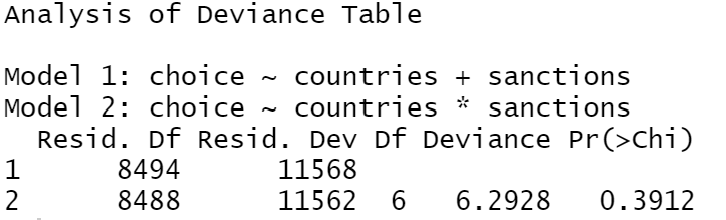
\includegraphics[width=.75\textwidth]{anova output.png}
	\end{figure} 
	
	\vspace{.5cm}
	As the p-value from the anova test (0.3912) is above our threshold of $\alpha$=0.05, we fail to reject the null hypothesis that the interactive model does not provide a better fit. Therefore, we do not have enough evidence to suggest that we should add an interactive term.
	
	\end{enumerate}
	\end{enumerate}


\end{document}
